\documentclass[a4paper,12pt]{article}
\usepackage[russian]{babel}
\usepackage[T2A]{fontenc}
\usepackage[utf8]{inputenc}
\usepackage{geometry}
\usepackage{amsmath}
\usepackage{graphicx}
\usepackage{cancel}
\usepackage{float} 
\usepackage{xcolor}
\usepackage{array}
\usepackage{caption}
\usepackage{booktabs}
\usepackage{amssymb}
\usepackage{subcaption}
\usepackage{pgfplots}
\pgfplotsset{compat=1.18}
\usetikzlibrary{arrows.meta, matrix}
\usepackage{capt-of}
\usepackage{multirow}
\usepackage[siunitx]{circuitikz}
\usepackage[bottom]{footmisc}
\usepackage{tcolorbox}
\usepackage{nicematrix}
\usepackage{tikz}
\usetikzlibrary{positioning, arrows.meta}

% --- hyperref ОДИН РАЗ ---
\usepackage{hyperref}
\hypersetup{linktoc=page}
\hypersetup{
	colorlinks=true,
	linkcolor=red,
	citecolor=red,
	urlcolor=red,
	filecolor=red,
}

% --- Содержание ---
\usepackage{tocloft}
\usepackage{etoolbox}
\usepackage{hyperref}
\hypersetup{
	colorlinks=true,
	linkcolor=red,
	citecolor=red,
	urlcolor=red,
}

% Патчим \tableofcontents: текст строк — без ссылок и чёрный
% Это делается через замену \contentsline внутри TOC
\preto\tableofcontents{%
	\begingroup
	% Переопределяем contentsline так, чтобы текст был чёрным без ссылки,
	% а номер страницы — красной ссылкой
	\renewcommand{\contentsline}[4]{%
		\ifnum\pdfstrcmp{##1}{section}=0
		\vskip 4pt{\normalfont\color{black}##2}\nobreak\hfill
		{\normalfont\color{red}\hyperlink{##4}{##3}}\par
		\else\ifnum\pdfstrcmp{##1}{subsection}=0
		\vskip 2pt\hspace{1.5em}{\normalfont\color{black}##2}\nobreak\hfill
		{\normalfont\color{red}\hyperlink{##4}{##3}}\par
		\else
		\vskip 1pt\hspace{3em}{\normalfont\color{black}##2}\nobreak\hfill
		{\normalfont\color{red}\hyperlink{##4}{##3}}\par
		\fi\fi
	}%
}
\appto\tableofcontents{\endgroup}

% tocloft — только для отступов, без переопределения шрифтов
\usepackage{tocloft}

% --- Листинги ---
\usepackage{listings}

\definecolor{codebg}{RGB}{250,250,252}
\definecolor{linenumcolor}{RGB}{150,150,170}
\definecolor{mathblue}{RGB}{30,100,200}
\definecolor{mathorange}{RGB}{200,100,20}
\definecolor{matlabblue}{RGB}{0,0,200}
\definecolor{matlabgreen}{RGB}{30,130,30}
\definecolor{matlaborange}{RGB}{200,80,0}

\lstdefinelanguage{Mathematica}{
	keywords={Plot, Eigenvalues, MatrixExp, RiccatiSolve, IdentityMatrix,
		Inverse, Transpose, Simplify, Eigensystem, StateSpaceModel,
		ControllabilityMatrix, MatrixRank, Export, FileNameJoin,
		NotebookDirectory, ConstantArray, ZeroMatrix, NDSolve,
		Evaluate, LineLegend, Placed, Directive, Opacity, Filling,
		FillingStyle, PlotStyle, PlotLegends, PlotRange, Frame,
		Axes, FrameLabel, GridLines, GridLinesStyle, AspectRatio,
		Style, FontFamily, FontSize, Thick, Dashed, Dotted,
		DotDashed, RGBColor, GrayLevel, LegendLayout, LabelStyle,
		Subscript, Table, Do, Module, Block, If, True, False, Automatic},
	sensitive=true,
	morecomment=[s]{(*}{*)},
	morestring=[b]",
}

\lstdefinestyle{mma}{
	language=Mathematica,
	basicstyle=\ttfamily\small,
	keywordstyle=\color{mathblue}\bfseries,
	commentstyle=\color{linenumcolor}\itshape,
	stringstyle=\color{mathorange},
	numberstyle=\tiny\color{linenumcolor},
	numbers=left,
	numbersep=10pt,
	backgroundcolor=\color{codebg},
	frame=single,
	frameround=tttt,
	framesep=4pt,
	rulecolor=\color{mathblue!40},
	breaklines=true,
	tabsize=4,
	showstringspaces=false,
	captionpos=b,
	xleftmargin=15pt,
	xrightmargin=5pt,
}

\lstdefinestyle{matlab}{
	language=Matlab,
	basicstyle=\ttfamily\small,
	keywordstyle=\color{matlabblue}\bfseries,
	commentstyle=\color{matlabgreen}\itshape,
	stringstyle=\color{matlaborange},
	numberstyle=\tiny\color{linenumcolor},
	numbers=left,
	numbersep=10pt,
	backgroundcolor=\color{codebg},
	frame=single,
	frameround=tttt,
	framesep=4pt,
	rulecolor=\color{matlabblue!30},
	breaklines=true,
	tabsize=4,
	showstringspaces=false,
	captionpos=b,
	xleftmargin=15pt,
	xrightmargin=5pt,
	escapeinside={\%*}{*)},
	morekeywords={cvx_begin,cvx_end,sdp,variable,minimize,maximize},
}

\lstset{style=mma}

\renewcommand{\lstlistingname}{Листинг}
\DeclareCaptionFormat{redlisting}{#1\textcolor{red}{#2}#3}
\captionsetup[lstlisting]{format=redlisting}

\geometry{left=1.5cm, right=2cm, bottom=2cm, top=2cm}
\captionsetup[figure]{name=Рисунок}
\captionsetup[table]{name=Таблица}
\captionsetup{labelsep=endash}


\begin{document}
	
	\begin{titlepage}
		\centering
		
		\vspace*{0.5cm}
		{\small
			Министерство науки и высшего образования Российской Федерации\\[2pt]
			Федеральное государственное автономное образовательное учреждение\\
			высшего образования\\[2pt]
			\textbf{«Национальный исследовательский университет ИТМО»}\\
		}
		
		\vspace{0.8cm}
		\hrule height 0.8pt
		\vspace{0.3cm}
		
		{\large Факультет систем управления и робототехники}
		
		\vspace{0.3cm}
		\hrule height 0.4pt
		\vspace{2.5cm}
		
		{\Huge\bfseries ОТЧЁТ}\\[0.4cm]
		{\LARGE\bfseries о лабораторной работе}\\[0.8cm]
		
		\begin{tcolorbox}[
			colback=gray!4,
			colframe=gray!10,
			boxrule=0.8pt,
			arc=4pt,
			left=12pt, right=12pt, top=8pt, bottom=8pt
			]
			\centering
			{\large По дисциплине:\\[4pt]}
			{\large\bfseries «Теория опимального управления»}\\[10pt]
			{\large Тема:\\[4pt]}
			{\large\bfseries «Синтез оптимального управления. Принцип максимума»} \\[10pt]
			{\large Поток: 1.3 \( \) Вариант: 18}
		\end{tcolorbox}
		
		\vspace{3cm}
		
		\begin{minipage}{0.45\textwidth}
			\raggedright
			{\large\bfseries Студент:}\\[4pt]
			Охрименко Е.\,Д.\\
		\end{minipage}
		\hfill
		\begin{minipage}{0.45\textwidth}
			\raggedleft
			{\large\bfseries Преподаватели:}\\[4pt]
			Герасимов Д.Н.\\
			Паромонов А. В.
		\end{minipage}
		
		\vfill
		\vspace{0.4cm}
		{\large Санкт-Петербург, 2026}
	\end{titlepage}
	
	\newpage
	\tableofcontents
	
	\newpage 

\section{Постановка задачи оптимального управления}

Рассмотрим задачу синтеза оптимального управления для линейного объекта на фиксированном интервале времени $T=9$ с закрепленными граничными условиями.

Математическая модель объекта:
\begin{equation}
	\begin{cases}
		\dot{x}_1 = x_2 \\
		\dot{x}_2 = -5x_2 + u
	\end{cases}
\end{equation}

Граничные условия:
\begin{equation}
	x_1(0) = 0 \qquad x_2(0) = 0 \qquad x_1(9) = 1 \qquad x_2(9) = 0
\end{equation}

Критерием качества является минимизация интегрального функционала:
\begin{equation}
	J = \int_{0}^{9} 5u^2(\tau) d\tau
\end{equation}

Требуется найти закон управления $u^*(t)$, удовлетворяющий принципу максимума, и промоделировать переходный процесс замкнутой системы.

\newpage
\section{Расчет оптимального управления}

Запишем гамильтониан ($\varphi_0 = -1$):

\[
\begin{aligned}
	H &= \varphi_0 u^2 + \varphi \dot x \\
	&= -5u^2 + \varphi_1 \dot x_1 + \varphi_2 \dot x_2 \\
	&= -5u^2 + \varphi_1 x_2 + \varphi_2 (-5 x_2 + u) \\
	&= -5 u^2 + x_2 (\varphi_1 - 5 \varphi_2) + \varphi_2 u
\end{aligned}
\]


Составим ситему уравнений Эйлера--Лагранжа:

\[
\begin{cases}
	\dot \varphi_i = - \dfrac{\partial H}{\partial x_i} \\[8pt]
	\dfrac{\partial H}{\partial u} = 0
\end{cases} \qquad \Longrightarrow \qquad 
\begin{cases}
    \dot{\varphi}_1 = 0,\\[6pt]
\dot{\varphi}_2 = 5\varphi_2 - \varphi_1 \\[6pt]
u^*(t) = \dfrac{\varphi_2(t)}{10}
\end{cases}
\]

Полная система дифференциальных уравнений замкнутой системы имеет вид:
\[
\begin{cases}
	\dot{x}_1 = x_2 \\[6pt]
	\dot{x}_2 = -5x_2 + \dfrac{\varphi_2}{10} \\[6pt]
	\dot{\varphi}_1 = 0 \\[6pt]
	\dot{\varphi}_2 = 5\varphi_2 - \varphi_1
\end{cases}
\]

Поскольку граничные условия заданы на обоих концах, задача сводится к двухточечной краевой задаче. Начальные значения $\varphi_1(0)$ и $\varphi_2(0)$ находятся из условия попадания в целевое состояние при $t=9$. Определим начальные условия сопряженной системы (листинг \ref{lst:odu}):

\[
\begin{aligned}	
	\begin{cases}
		\varphi_1(0) &= \dfrac{1250 \left(1+e^{45}\right)}{47+43 e^{45}} \\[10pt]
		\varphi_2(0) &= -\dfrac{250 \left(1-e^{45}\right)}{47+43 e^{45}}
	\end{cases} \qquad \Longrightarrow \qquad
	\begin{cases}
		\varphi_1(0) &= 29.07 \\
		\varphi_2(0) &= 5.81
	\end{cases}
\end{aligned}
\]

\newpage
\section{Схема системы в Simulink}

Уравнения объекта управления:

\[
	\begin{cases}
		\dot{x}_1 = x_2 \\
		\dot{x}_2 = -5x_2 + u
	\end{cases}
\]

\begin{figure}[H]
	\centering
	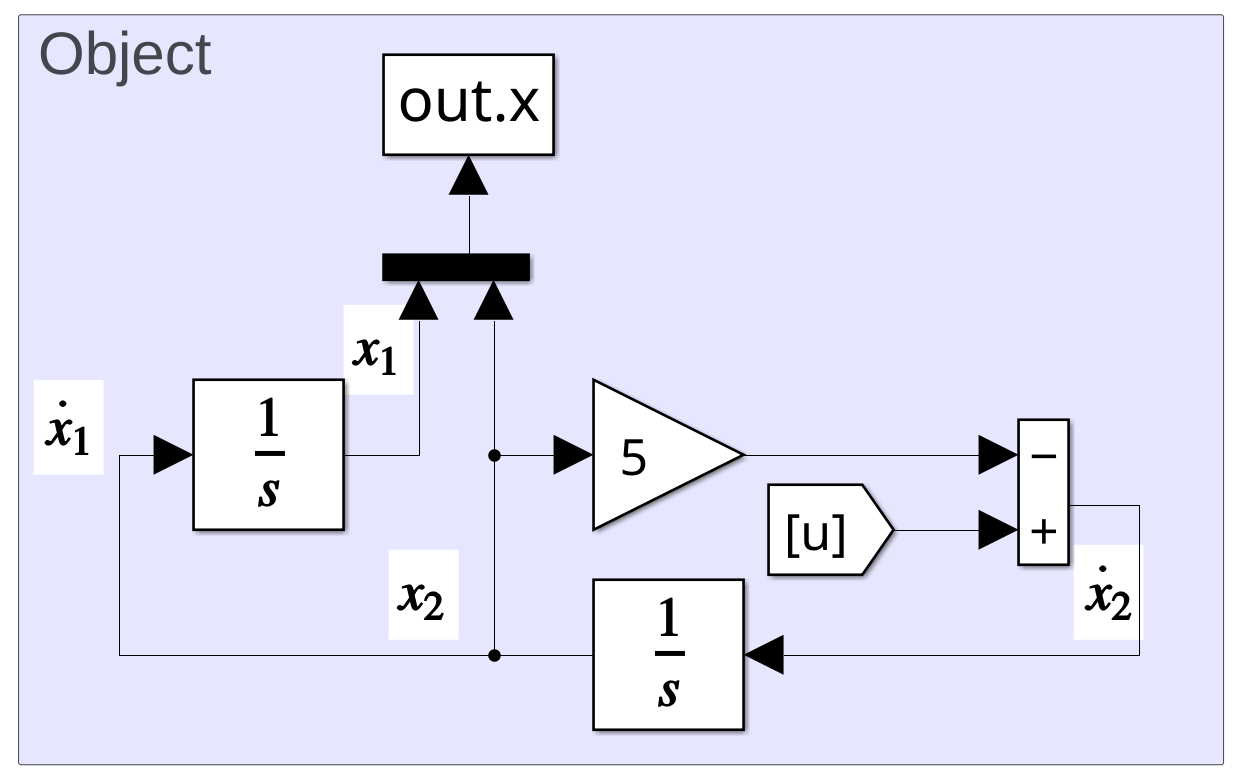
\includegraphics[width=0.45\textwidth]{../images/obj.png}
	\caption{Схема моделирования объекта управления}
\end{figure}

Уравнения сопряженной системы:

\[
\begin{cases}
	\dot{\varphi}_1 = 0 \\[6pt]
	\dot{\varphi}_2 = 5\varphi_2 - \varphi_1
\end{cases}
\]

\begin{figure}[H]
	\centering
	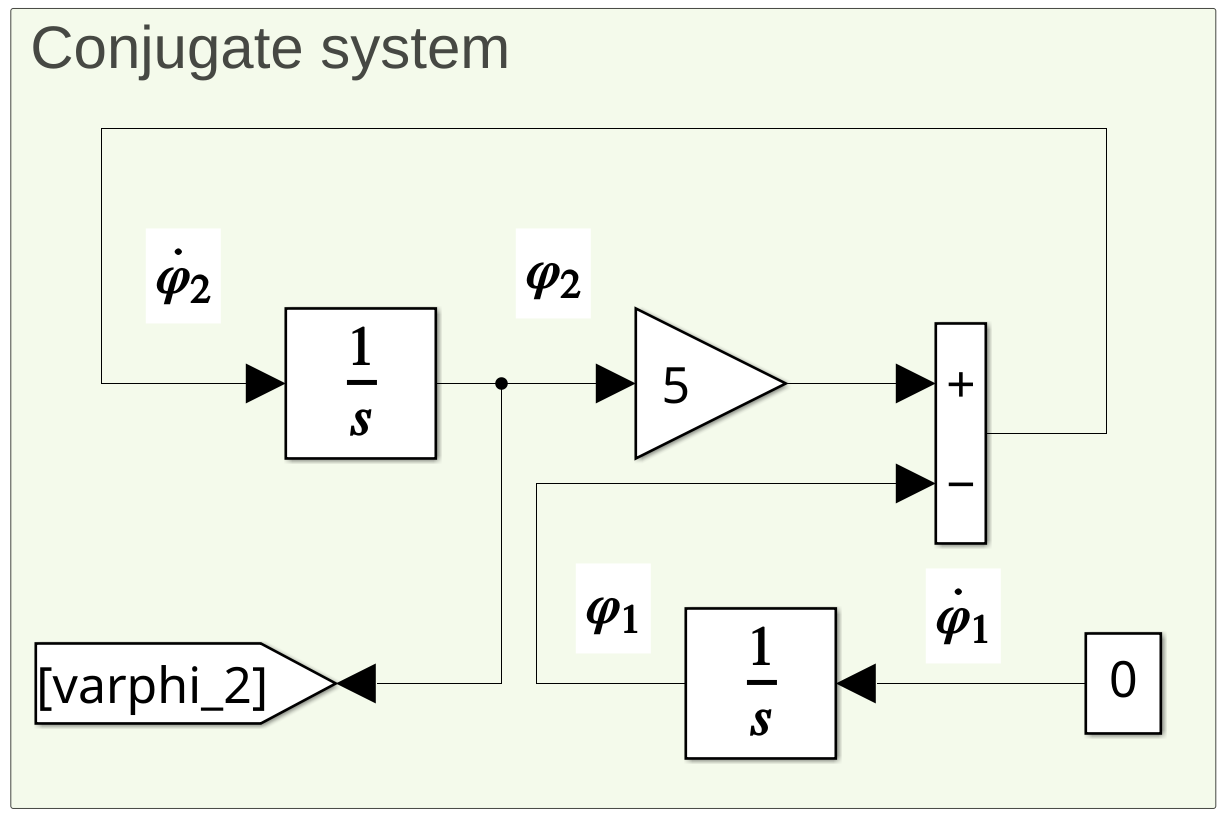
\includegraphics[width=0.45\textwidth]{../images/Conjugate.png}
	\caption{Схема моделирования сопряженной системы}
\end{figure}

Функционал качества:


\[	J = \int_{0}^{9} 5u^2(\tau) d\tau\]


\begin{figure}[H]
	\centering
	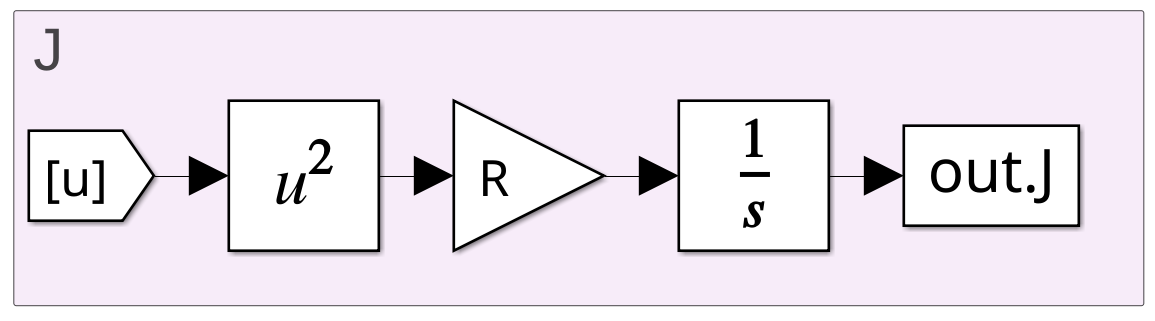
\includegraphics[width=0.45\textwidth]{../images/J.png}
	\caption{Схема моделирования функционал качества}
\end{figure}

	
Оптимальное управление:

	
\[u^*(t) = \dfrac{\varphi_2(t)}{10}\]	
	
\begin{figure}[H]
	\centering
	\includegraphics[width=0.45\textwidth]{../images/Control.png}
	\caption{Схема моделирования управления}
\end{figure}
	

\newpage
\section{Моделирование системы}

Численное моделирование в Simulink выполнено с решателем \texttt{ode15s} и жесткими допусками ($\varepsilon_{rel}=10^{-10}$, $\Delta t_{max}=0.01$). Из-за накопления вычислительных погрешностей результаты численного интегрирования отличаются от аналитических, поэтому далее представлены графики, построенные двумя способами.

\begin{figure}[H]
	\centering
	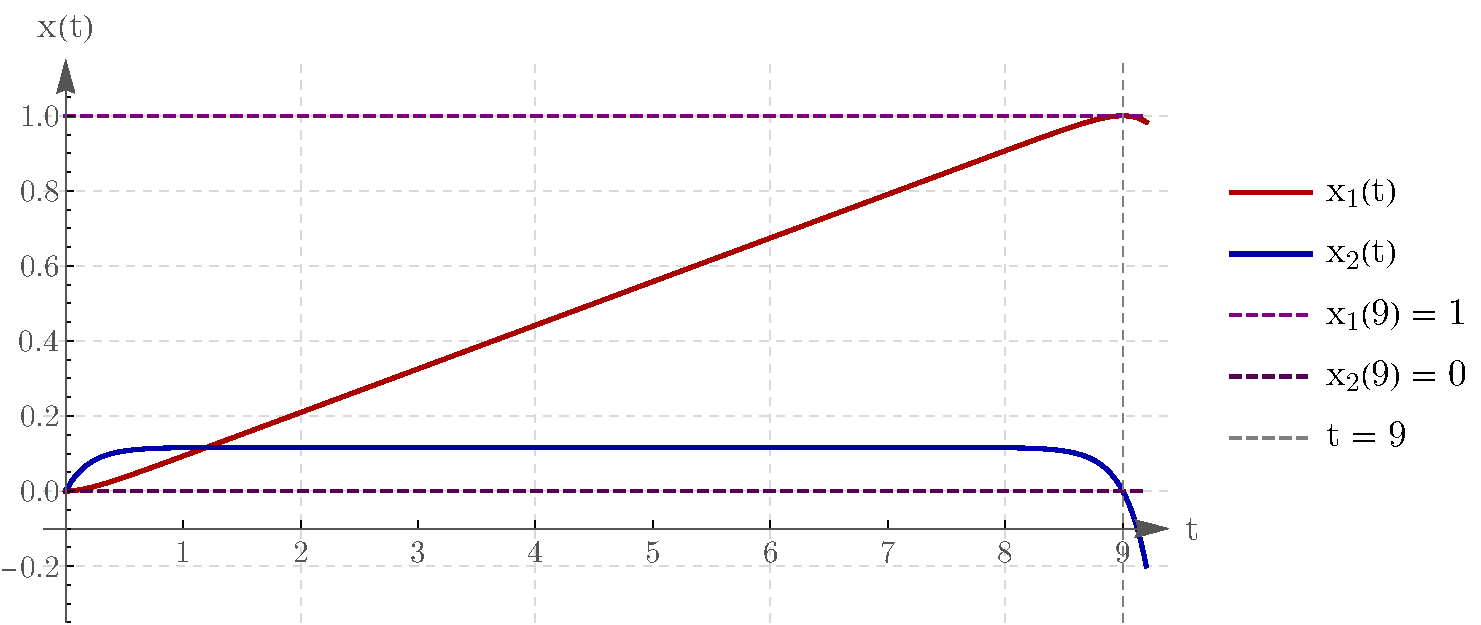
\includegraphics[width=0.7\textwidth]{../images/x.pdf}
	\caption{Траектории компонент вектора состояния \(x(t)\)}
	\label{fig:x_math}
\end{figure}

\begin{figure}[H]
	\centering
	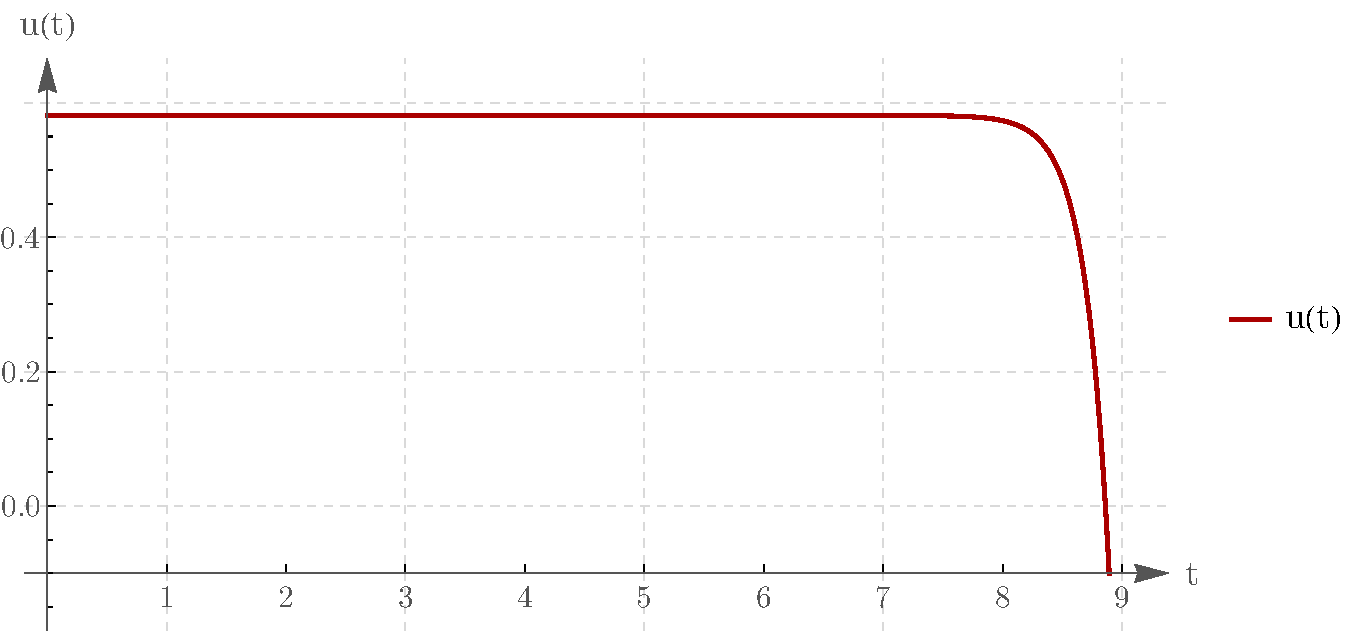
\includegraphics[width=0.7\textwidth]{../images/u.pdf}
	\caption{Оптимальное управление \(u(t)\)}
	\label{fig:u_math}
\end{figure}

\begin{figure}[H]
	\centering
	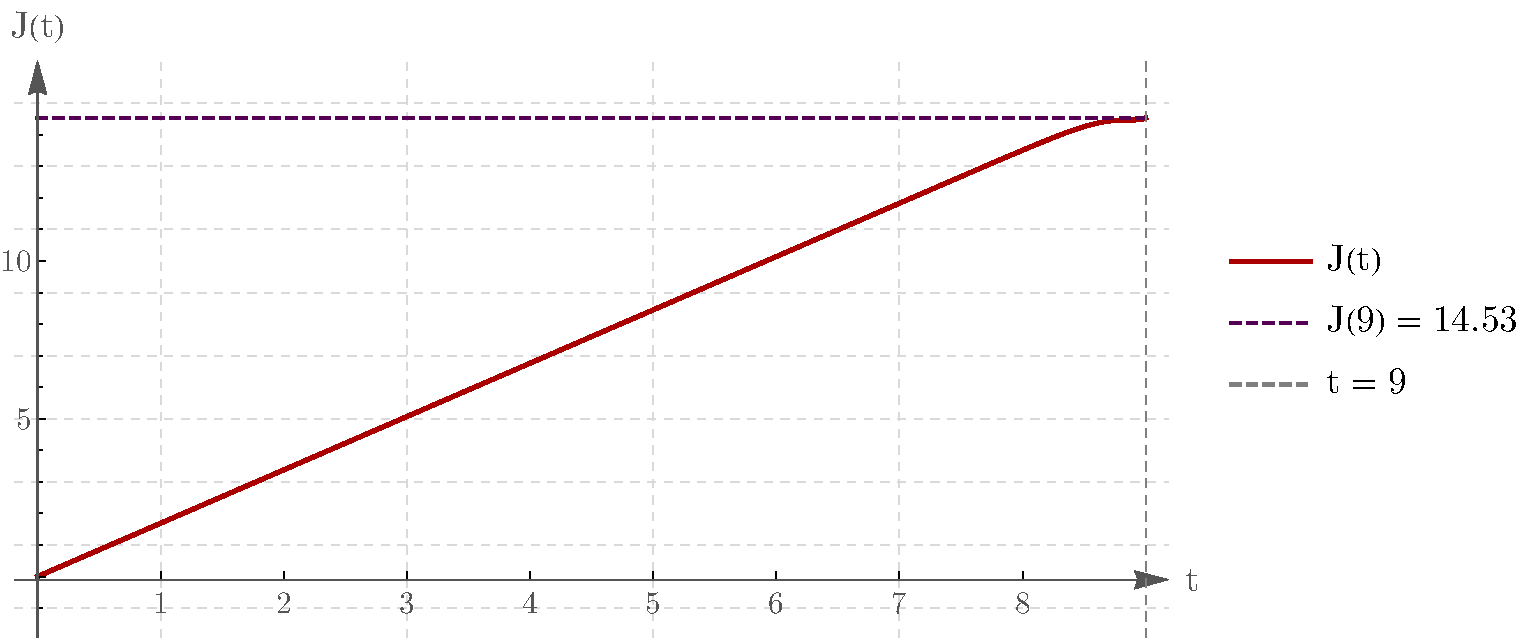
\includegraphics[width=0.7\textwidth]{../images/J.pdf}
	\caption{Критерий качества \(J(t)\)}
	\label{fig:J_math}
\end{figure}

\newpage

\begin{figure}[H]
	\centering
	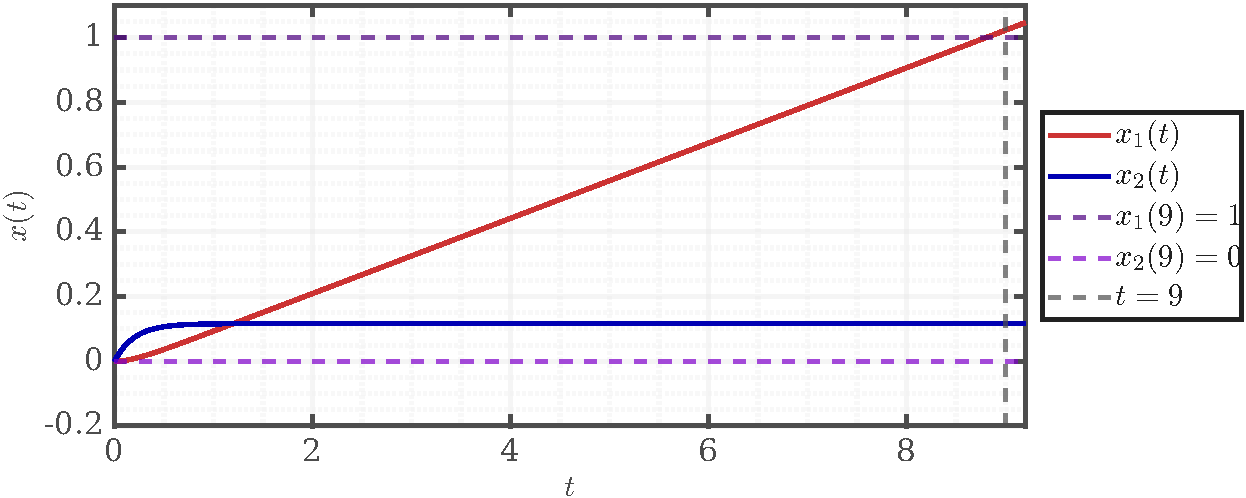
\includegraphics[width=0.7\textwidth]{../images/x_sim.pdf}
	\caption{Траектории компонент вектора состояния \(x(t)\) (Simulink)}
	\label{fig:x_sim}
\end{figure}

\begin{figure}[H]
	\centering
	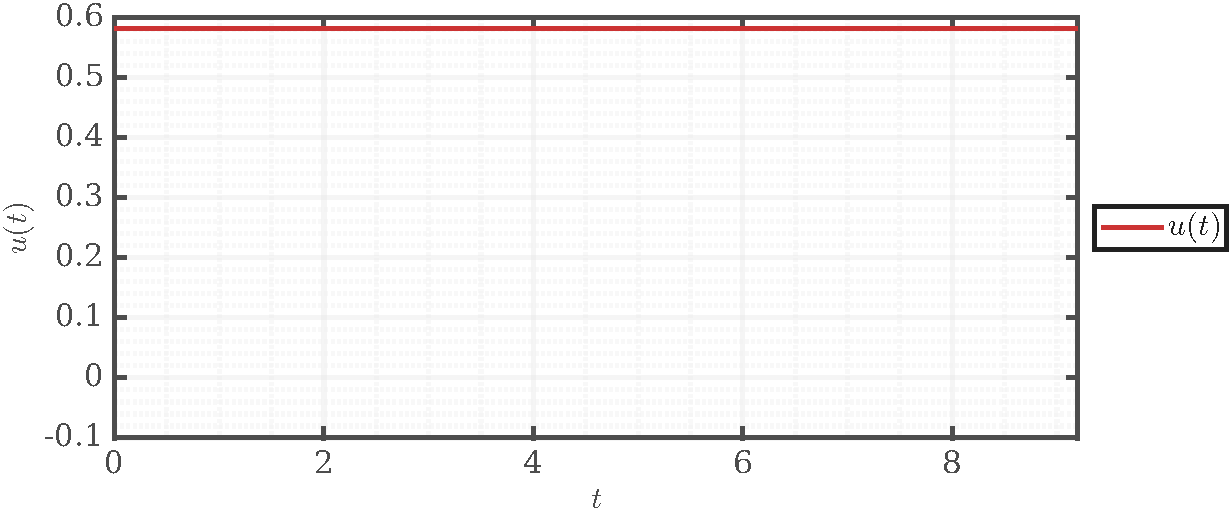
\includegraphics[width=0.7\textwidth]{../images/u_sim.pdf}
	\caption{Управление \(u(t)\) (Simulink)}
	\label{fig:u_sim}
\end{figure}

\begin{figure}[H]
	\centering
	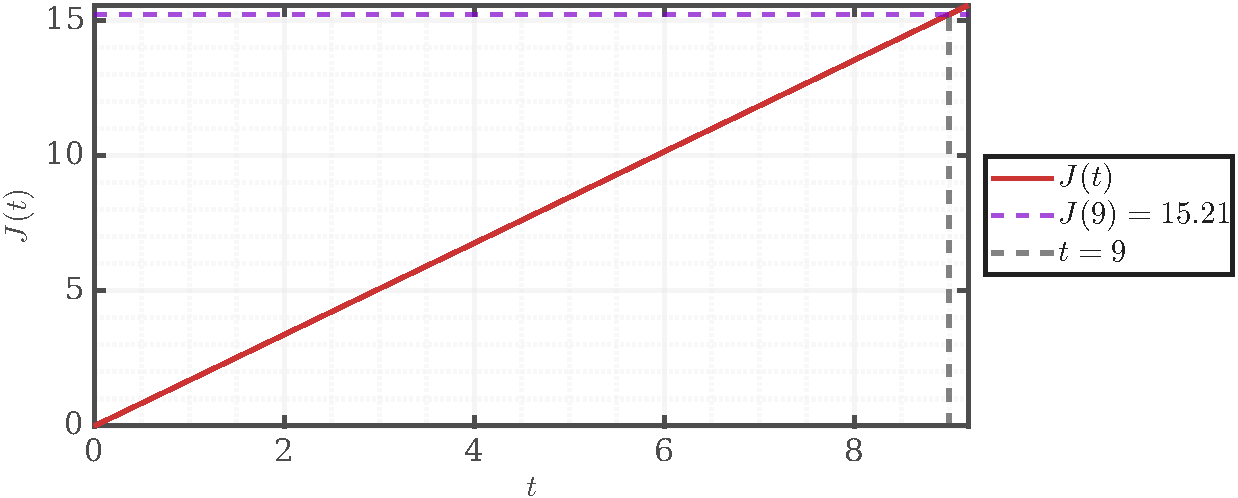
\includegraphics[width=0.7\textwidth]{../images/J_sim.pdf}
	\caption{Критерий качества \(J(t)\) (Simulink)}
	\label{fig:J_sim}
\end{figure}
	
	
	
	При прямом интегрировании синтезированной системы в Simulink траектория не достигла целевого состояния: к моменту $t=9$ наблюдаются отклонения $x_1(9) \approx 1.02$ и $x_2(9) \approx 0.12$. А также значение критерия качества $J_{sim}$ оказалось выше эталонного значения $J^*$, полученного аналитически.
	

	\newpage
	\section{Расчет критерия качества при отклонении параметров регулятора от оптимальных значений}

При отклонении начальных условий сопряженной системы $\varphi(0)$ на $\pm 10\%$ от оптимальных значений получены следующие выражения накопленного критерия качества:
	
	\[
		J_{-10\%}(t) = 1.3690 \cdot t \qquad 
		J_{+10\%}(t) = 2.0450 \cdot t
	\]
	
	Подставляя $T=9$, получаем итоговые значения функционала:
	\[
	J_{-10\%}(9) \approx 12.32 \qquad 
	J_{+10\%}(9) \approx 18.41
	\]
	
		
	Для оценки чувствительности синтезированного управления было проведено моделирование. Результаты представлены на рисунке~\ref{fig:J_deviation}.
	
	\begin{figure}[H]
		\centering
		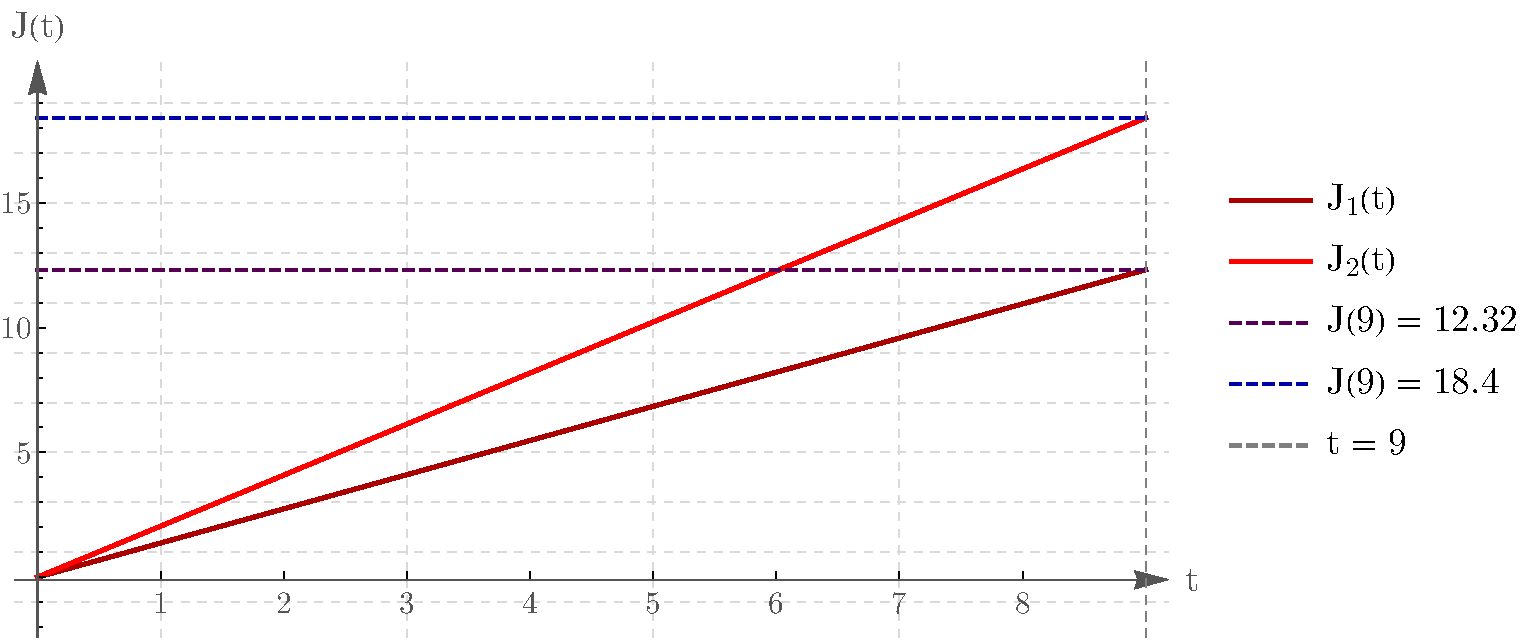
\includegraphics[width=0.7\textwidth]{../images/J12.pdf} 
		\caption{Динамика критерия качества $J(t)$ при отклонении параметров регулятора на $\pm 10\%$}
		\label{fig:J_deviation}
	\end{figure}
	
	Как видно из графика, даже незначительное изменение параметров приводит к существенному изменению значения функционала. При отклонении $-10\%$ наблюдается снижение накопленного критерия $J$. При отклонении $+10\%$ значение $J$ возрастает. Это подтверждает высокую чувствительность оптимального регулятора к точности задания начальных условий сопряженных переменных.
	
	
	\newpage
	\section{Вывод}
	
	Синтезированное на основе принципа максимума оптимальное управление обеспечивает точное выполнение граничных условий и минимальные затраты управления при строгом соблюдении начальных условий сопряженной системы.
	
	
	
	
	
	
	

	
\newpage
\section{Приложение}

\begin{lstlisting}[caption={Решение ОДУ}, label=lst:odu]
T = 9;

sol = DSolve[
	{
		x1'[t] == x2[t],
		x2'[t] == -5 x2[t] + phi2[t]/10,
		
		phi1'[t] == 0,
		phi2'[t] == -phi1[t] + 5 phi2[t],
		
		x1[0] == 0, x2[0] == 0,
		x1[T] == 1, x2[T] == 0
	},
	
	{x1, x2, phi1, phi2}, t
];

psi1_opt = phi1[0] /. sol[[1]]
psi2_opt = phi2[0] /. sol[[1]]
\end{lstlisting}
	
\end{document}